\iffalse
\let\negmedspace\undefined
\let\negthickspace\undefined
\documentclass[journal,12pt,twocolumn]{IEEEtran}
\usepackage{cite}
\usepackage{amsmath,amssymb,amsfonts,amsthm}
\usepackage{algorithmic}
\usepackage{graphicx}
\usepackage{textcomp}
\usepackage{xcolor}
\usepackage{txfonts}
\usepackage{listings}
\usepackage{enumitem}
\usepackage{mathtools}
\usepackage{gensymb}
\usepackage{comment}
\usepackage[breaklinks=true]{hyperref}
\usepackage{tkz-euclide}
\usepackage{listings}
\usepackage{gvv}
\def\inputGnumericTable{}
\usepackage[latin1]{inputenc}
\usepackage{color}
\usepackage{array}
\usepackage{longtable}
\usepackage{calc}
\usepackage{multirow}
\usepackage{hhline}
\usepackage{ifthen}
\usepackage{lscape}

\newtheorem{theorem}{Theorem}[section]
\newtheorem{problem}{Problem}
\newtheorem{proposition}{Proposition}[section]
\newtheorem{lemma}{Lemma}[section]
\newtheorem{corollary}[theorem]{Corollary}
\newtheorem{example}{Example}[section]
\newtheorem{definition}[problem]{Definition}
\newcommand{\BEQA}{\begin{eqnarray}}
\newcommand{\EEQA}{\end{eqnarray}}
\newcommand{\define}{\stackrel{\triangle}{=}}
\theoremstyle{remark}
\newtheorem{rem}{Remark}
\begin{document}

\bibliographystyle{IEEEtran}
\vspace{3cm}

\title{NCERT Analog Assignment}
\author{EE23BTECH11007 - Aneesh Kadiyala$^{*}$% <-this % stops a space
}
\maketitle
\newpage
\bigskip

\renewcommand{\thefigure}{\theenumi}
\renewcommand{\thetable}{\theenumi}

\vspace{3cm}
\textbf{Question 11.14.17:} A simple pendulum of length $\ell$ and having a bob of mass $M$ is suspended in a car. The car is moving in a circular track of radius $R$ with a uniform speed $v$. If the pendulum makes small oscillations in a radial direction about its equilibrium position, what will be its time period?
\\
\solution
\fi
\begin{table}[h!]
    \centering
    \begin{tabular}{ | c | c | }
    \hline
    Parameter & Description \\
    \hline
    $v$ & Speed \\
    \hline
    $R$ & Radius of circular track \\
    \hline
    $M$ & Mass of bob \\
    \hline
    $g$ & Acceleration due to gravity \\
    \hline
    $a_c$ & Centrifugal acceleration \\
    \hline
    $g_e$ & Effective gravitational acceleration $\sqrt{g^2 + a^2}$ \\
    \hline
    Residual Formula for $m = 1$ & $\lim_{s \to a}\brak{\brak{s - a}\theta\brak{t}e^{st}}$\\
    \hline
\end{tabular}
    \caption{Parameters}
    \label{tab:physics-11-14-17}
\end{table}
\begin{figure}[h!]
\centering
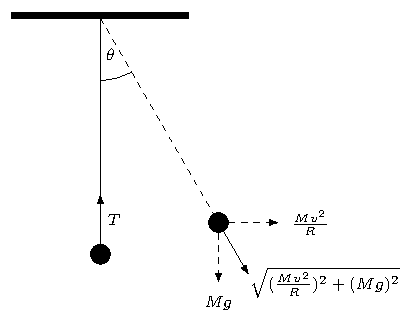
\includegraphics{ncert-physics/11/14/17/figs/fbd.pdf}
\caption{Free Body Diagram}
\label{fig:analog_11_14_17_1}
\end{figure}

From the figure, restoring force:
\begin{align}
F_r &= -\brak{\sqrt{\brak{\frac{Mv^2}{R}}^2+\brak{Mg}^2}}\sin{\theta\brak{t}}
\end{align}
For small oscillations, $\theta\brak{t} << 1$.
\begin{align}
\implies \sin{\theta\brak{t}} &\approx \theta\brak{t} \\
\implies F_r &\approx -\brak{\sqrt{\brak{\frac{Mv^2}{R}}^2+\brak{Mg}^2}}\theta\brak{t} \\
\implies a &= -\brak{\sqrt{\brak{\frac{v^2}{R}}^2+g^2}}\theta\brak{t} \\
l\frac{d^2\theta\brak{t}}{dt^2} &= -\brak{\sqrt{\brak{\frac{v^2}{R}}^2+g^2}}\theta\brak{t} \\
\text{Let } k &= \frac{1}{\ell}\brak{\sqrt{\brak{\frac{v^2}{R}}^2+g^2}} \\
\frac{d^2\theta\brak{t}}{dt^2} + k\theta\brak{t} &= 0 \\
\end{align}
Taking Laplace transform:
\begin{align}
s^2\Theta\brak{s} - s\theta(0) - \theta'(0) + k\Theta\brak{s} &= 0
\end{align}
Assuming $\theta(0) = 0$:
\begin{align}
s^2\Theta\brak{s} - \theta'(0) + k\Theta\brak{s} &= 0 \\
\implies \Theta\brak{s} &= \frac{\theta'(0)}{s^2 + k}
\end{align}
Taking inverse laplace transform using Bromwich integral:
\begin{align}
\theta(t) &= \frac{1}{2\pi j}\int_{c-j\infty}^{c+j\infty}\Theta(s)e^{st}dt, c > 0 \\
&= \frac{1}{2\pi j}\int_{c-j\infty}^{c+j\infty}\frac{\theta'(0)e^{st}}{s^2 + k}dt
\end{align}
Since the poles $s=j\sqrt{k}$ and $s=-j\sqrt{k}$ (both non repeated, i.e. $m=1$) lie inside a semicircle for some $c>0$. Using Jordans lemma and method of residues from \ref{tab:physics-11-14-17}:
\begin{align}
R_1&=\lim\limits_{s\to j\sqrt{k}}\brak {{\brak{s-j\sqrt{k}}}\brak{\frac{\theta'(0)}{s^2+k}} e^{st}}\\
&={\brak{\frac{\theta'(0)e^{j\sqrt{k}t}}{2j\sqrt{k}}}}\\
R_2&=\lim\limits_{s\to -j\sqrt{k}}\brak {{\brak{s+j\sqrt{k}}}\brak{\frac{\theta'(0)}{s^2+k}} e^{st}}\\
&={\brak{\frac{-\theta'(0)e^{-j\sqrt{k}t}}{2j\sqrt{k}}}}\\
\theta(t) &= R_1 + R_2\\
\theta(t) &= {\brak{\frac{\theta'(0)\brak{e^{j\sqrt{k}t}-e^{-j\sqrt{k}t}}}{2j\sqrt{k}}}}\\
\implies
\theta(t) &=\frac{\theta'(0)}{\sqrt{k}}\sin{\brak{\sqrt{k}t}} \\
\implies \theta(t) &= \frac{\theta'(0)}{\sqrt{\frac{1}{\ell}\brak{\sqrt{\brak{\frac{v^2}{R}}^2+g^2}}}}\sin{\brak{\sqrt{\frac{1}{\ell}\brak{\sqrt{\brak{\frac{v^2}{R}}^2+g^2}}}t}}
\end{align}
\begin{figure}[h!]
\centering
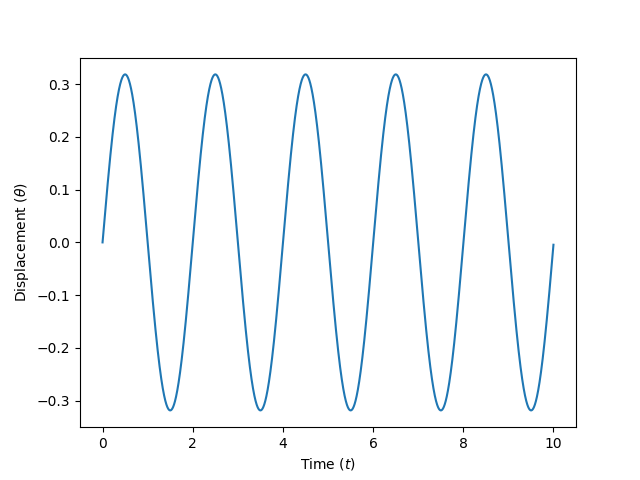
\includegraphics[width=\columnwidth]{ncert-physics/11/14/17/figs/plot.png}
\caption{$\theta\brak{t}$ vs $t$ for $v = 1, R = 1, \ell = 1, g = 9.8, \theta'\brak{0} = 1$}
\label{fig:analog_11_14_17_2}
\end{figure}
\begin{align}
\frac{2\pi}{T} &= \sqrt{\frac{1}{\ell}\brak{\sqrt{\brak{\frac{v^2}{R}}^2+g^2}}} \\
\implies T &= 2\pi\sqrt{\frac{\ell}{\sqrt{\brak{\frac{v^2}{R}}^2+g^2}}}
\end{align}